%!TEX program = xelatex
\let\stop\empty

\documentclass[12pt,a4paper]{exam-zh}

% ==========================
% 卷面变量设置（只需改这里）
% ==========================
% ==========================
% 卷面变量设置（只需改这里）
% ==========================
\newcommand{\paperlevel}{高中一}
\newcommand{\papersubject}{数学 试卷二}
\newcommand{\schoolname}{金宝培元独立中学}
\newcommand{\examname}{年终考}
\newcommand{\classinfo}{S1(Y / H)}
\newcommand{\examdate}{3-11-2026}
\newcommand{\examtime}{12:55-14:10}
\newcommand{\questiontotal}{8}
\newcommand{\paperpercentage}{70\%}
\newcommand{\setterteacher}{蔡杰庆师}
\newcommand{\reviewteacher}{王萌师}
\newcommand{\auditteacher}{雷泳健师}


\usepackage{xeCJK}
% \setCJKmainfont{NSimSun}
\setCJKmainfont{Noto Serif CJK SC}
\usepackage{geometry}
\usepackage{array}
\usepackage{tikz}
\usepackage{amsmath}
\usepackage{wrapfig}
\usepackage{adjustbox}
\usepackage{enumitem}
\usepackage{fancyhdr}
\usetikzlibrary{quotes,angles}
\usetikzlibrary{calc}
\usepackage{scalerel}
\def\mcirc{\mathbin{\scalerel*{\circ}{j}}}
\def\msquare{\mathord{\scalerel*{\Box}{gX}}}

% \renewcommand{\choiceshook}{%
%     \setlength{\leftmargin}{18pt}%
% }
\AtBeginDocument{%
    \zihao{4}%
}


%region ----------- 调整 exam -----------
\examsetup{
    % problem/label = \arabic*., 
    % 设置大题题号格式 
        problem = {
        top-sep = 1em,      % 题头上方的间距（默认 0.25em）
        bottom-sep = 1em,   % 题号下方的间距（默认 0pt）
    },
    % 隐藏大题后的分值显示 
    problem/show-points = false,
    % 调整各 question 之间的垂直间距
    question = {
        top-sep = 1em,
        bottom-sep = 1em,
    },
    % 调整小题列表的缩进和间距
    list/step-name = {}, 
    solution = {
    show-solution = show-move, % 答案自动移动到卷末
    label-content = {参考答案},  % 答案区的标题文字
    show-qed = true            % 在解答末尾显示结束符号 ◻ 
  },
    page = {
    size = a4paper,           % 设定纸张大小 
    foot-content = { - ; - }  % 页脚显示为 -1-, -2- 格式 
  }
}
\setlist[enumerate,1]{
    label=(\alpha*), 
    itemsep=0.5em, 
    leftmargin=2em, 
    after=\hfill % 配合您之前要求的百分比靠右样式
}
%endregion

\newcommand{\qscoreoffset}{0em}
\newlist{questionparts}{enumerate}{1}
\setlist[questionparts]{
    label=(\alph*),
    itemsep=0.5em,
    leftmargin=2em,
    rightmargin=4em,
    before={\renewcommand{\qscoreoffset}{4em}},
}
\newcommand{\qscore}[2][\%]{%
    \leavevmode\unskip\nobreak\hfill
    \makebox[0pt][l]{\makebox[\qscoreoffset][r]{(#2#1)}}%
}

\newcommand{\makeexamheader}{%
%region 三栏标题区
% ==========================
\noindent
\begin{tabular*}{\textwidth}{@{\extracolsep{\fill}} p{0.3\textwidth} p{0.35\textwidth} p{0.3\textwidth}}

\raggedright
\textbf{\paperlevel}\\[0.2em]
\textbf{}{\papersubject}\\[0.4em]
姓名：\underline{\hspace{3cm}} &

\centering
\textbf{\schoolname}\\[0.2em]
\textbf{\examname}\\[0.4em]
班级：\classinfo &

\raggedright
日期：\examdate\\[0.2em]
时间：\examtime\\[0.4em]
得分：\underline{\hspace{2.5cm}} \\

\end{tabular*}

\begin{flushleft}
作答题：\questiontotal 题全做（\paperpercentage） 
\end{flushleft}
%endregion
}

\begin{document}
\makeexamheader
% 需要的宏包/库：exam-zh；\usetikzlibrary{angles,quotes}
% 作答题 8 题，共 70 分：6+6+6+8+8+8+14+14

%region 范围：第 9 章 任意角的三角函数 | 考点：9.1+9.2 诱导公式化简求值（含特殊角） | 难度：易
\begin{question}[points = 6]
    已知
       $f(\alpha)=\dfrac{\sin(180^{\circ}-\alpha)\cos(360^{\circ}-\alpha)\tan(180^{\circ}+\alpha)}{\cos(90^{\circ}+\alpha)\sin(270^{\circ}+\alpha)}$。 
    \begin{questionparts}
        \item 化简 $f(\alpha)$。 \qscore{3}

        \item 求 $f(-1020^{\circ})$ 的值。 \qscore{3}
    \end{questionparts}
\end{question}

\begin{solution}
    \begin{enumerate}[label=(\alph*)]
        \item 化简 $f(\alpha)$。 \\
        分别用诱导公式化简分子、分母，再约分。 \\
        \begin{align*}
            \sin(180^{\circ}-\alpha)\cos(360^{\circ}-\alpha)\tan(180^{\circ}+\alpha) &= \sin\alpha\cos\alpha\tan\alpha
        \end{align*}
        \begin{align*}
            \cos(90^{\circ}+\alpha)\sin(270^{\circ}+\alpha) &= (-\sin\alpha)(-\cos\alpha) = \sin\alpha\cos\alpha
        \end{align*}
        \begin{align*}
            f(\alpha) &= \frac{\sin\alpha\cos\alpha\tan\alpha}{\sin\alpha\cos\alpha} = \tan\alpha
        \end{align*}

        \item 求 $f(-1020^{\circ})$ 的值。 \\
        由 (a) 知 $f(\alpha)=\tan\alpha$，再用诱导公式化为特殊角。 \\
        \begin{align*}
            f(-1020^{\circ}) &= \tan(-1020^{\circ}) = -\tan 1020^{\circ}
        \end{align*}
        \begin{align*}
            -\tan 1020^{\circ} &= -\tan(2\times 360^{\circ}+300^{\circ}) = -\tan 300^{\circ}
        \end{align*}
        \begin{align*}
            -\tan 300^{\circ} &= -\tan(360^{\circ}-60^{\circ}) = \tan 60^{\circ} = \sqrt{3}
        \end{align*}
    \end{enumerate}
\end{solution}
%endregion

%region 范围：第 9 章 任意角的三角函数 | 考点：9.3 图像的定义域、值域、五点法作图 | 难度：易
\begin{question}[points = 6]
    已知函数 $f(x)=\sin\left(x+\dfrac{\pi}{3}\right)-1$。
    \begin{questionparts}
        \item 求 $f(x)$ 的定义域与值域。 \qscore{3}

        \item 作出 $f(x)$ 在区间 $[-2\pi,\,2\pi]$ 上的简图。 \qscore{3}
    \end{questionparts}
\end{question}

\begin{solution}
    \begin{enumerate}[label=(\alph*)]
        \item 求 $f(x)=\sin\left(x+\frac{\pi}{3}\right)-1$ 的定义域与值域。 \\
        正弦函数的定义域为 $\mathbb{R}$；由 $-1\le\sin\left(x+\frac{\pi}{3}\right)\le 1$ 逐步变形求值域。 \\
        \[
            x\in\mathbb{R}
        \]
        \begin{align*}
            -1 \le \sin\left(x+\frac{\pi}{3}\right) \le 1 &\Rightarrow -2 \le \sin\left(x+\frac{\pi}{3}\right)-1 \le 0 \\
            &\Rightarrow f(x)\in[-2,\,0]
        \end{align*}

        \item 作 $f(x)=\sin\left(x+\frac{\pi}{3}\right)-1$ 在 $[-2\pi,\,2\pi]$ 上的简图。 \\
        令 $x+\frac{\pi}{3}=\frac{k\pi}{2}$ 得关键点，连同区间端点列表描点，再用光滑曲线连接。 \\
        \begin{center}
            \small
            \renewcommand{\arraystretch}{1.6}
            \setlength{\tabcolsep}{4pt}
            \begin{tabular}{c|cccccccccc}
                $x$ & $-2\pi$ & $-\dfrac{11\pi}{6}$ & $-\dfrac{4\pi}{3}$ & $-\dfrac{5\pi}{6}$ & $-\dfrac{\pi}{3}$ & $\dfrac{\pi}{6}$ & $\dfrac{2\pi}{3}$ & $\dfrac{7\pi}{6}$ & $\dfrac{5\pi}{3}$ & $2\pi$ \\ \hline
                $y$ & $\dfrac{\sqrt{3}}{2}-1$ & $0$ & $-1$ & $-2$ & $-1$ & $0$ & $-1$ & $-2$ & $-1$ & $\dfrac{\sqrt{3}}{2}-1$
            \end{tabular}
        \end{center}
        \begin{center}
            \begin{tikzpicture}[x=0.72cm, y=1.3cm, >=stealth]
                % 坐标轴
                \draw[->] (-7.2,0) -- (7.2,0) node[right] {$x$};
                \draw[->] (0,-2.6) -- (0,0.7) node[above] {$y$};
                \node[above right] at (0,0) {$O$};
                % y 轴刻度
                \foreach \y in {-1,-2} {
                    \draw (0,\y) -- (0.08,\y);
                    \node[left] at (0,\y) {$\y$};
                }
                % x 轴刻度（曲线位于 x 轴下方，标签放在上方）
                \foreach \x/\l in {-6.2832/{-2\pi}, -3.1416/{-\pi}, 3.1416/{\pi}, 6.2832/{2\pi}} {
                    \draw (\x,0) -- (\x,-0.08);
                    \node[above] at (\x,0) {$\l$};
                }
                % 曲线
                \draw[thick, smooth, samples=150, domain=-6.2832:6.2832, variable=\t]
                    plot ({\t},{sin((\t+1.0472) r)-1});
                % 关键点
                \foreach \x/\y in {-5.7596/0, -4.1888/-1, -2.6180/-2, -1.0472/-1,
                                   0.5236/0, 2.0944/-1, 3.6652/-2, 5.2360/-1} {
                    \fill (\x,\y) circle (1.5pt);
                }
                % 区间端点
                \fill (-6.2832,-0.134) circle (1.5pt);
                \fill (6.2832,-0.134) circle (1.5pt);
            \end{tikzpicture}
        \end{center}
    \end{enumerate}
\end{solution}
%endregion

%region 范围：第 11 章 三角恒等式与三角方程式 | 考点：11.1 三角恒等式的证明 | 难度：易
\begin{question}[points = 6]
    证明：$\dfrac{1-2\sin x\cos x}{\cos^2 x-\sin^2 x}=\dfrac{1-\tan x}{1+\tan x}$。
    \qscore{6}
\end{question}

\begin{solution}
    证明左边等于右边。 \\
    左边分子用 $1=\sin^2x+\cos^2x$ 配成完全平方，分母用平方差公式，约分后分子分母同除以 $\cos x$。 \\
    \begin{align*}
        1-2\sin x\cos x &= \sin^2x+\cos^2x-2\sin x\cos x = (\cos x-\sin x)^2
    \end{align*}
    \begin{align*}
        \cos^2x-\sin^2x &= (\cos x-\sin x)(\cos x+\sin x)
    \end{align*}
    \begin{align*}
        \text{左边} &= \frac{(\cos x-\sin x)^2}{(\cos x-\sin x)(\cos x+\sin x)} = \frac{\cos x-\sin x}{\cos x+\sin x}
    \end{align*}
    \begin{align*}
        \frac{\cos x-\sin x}{\cos x+\sin x} &= \frac{1-\tan x}{1+\tan x} = \text{右边}
    \end{align*}
\end{solution}
%endregion

%region 范围：第 9 章 任意角的三角函数 | 考点：9.2+9.5 二倍角公式、弦化切；9.4 反三角函数的图像、定义域与值域 | 难度：中
\begin{question}[points = 8]
    \begin{questionparts}
        \item 已知 $\dfrac{3\pi}{4}<\theta<\pi$，$\sin2\theta=-\dfrac{3}{5}$，求 $\tan\theta$ 的值。（不得使用计算器） \qscore{4}

        \item 作出函数 $y=\cos^{-1}x$ 的图像，并写出其定义域与值域。 \qscore{4}
    \end{questionparts}
\end{question}

\begin{solution}
    \begin{enumerate}[label=(\alph*)]
        \item 已知 $\frac{3\pi}{4}<\theta<\pi$，$\sin2\theta=-\frac{3}{5}$，求 $\tan\theta$。 \\
        将 $\sin2\theta$ 化为关于 $\tan\theta$ 的式子，解方程后由 $\theta$ 的范围舍去增根。 \\
        设 $t=\tan\theta$。
        \begin{align*}
            \sin2\theta &= \frac{2\sin\theta\cos\theta}{\sin^2\theta+\cos^2\theta} = \frac{2t}{1+t^2} \\
            \frac{2t}{1+t^2} &= -\frac{3}{5} \\
            3t^2+10t+3 &= 0
        \end{align*}
        \begin{align*}
            (3t+1)(t+3) &= 0 \\
            t &= -\frac{1}{3}\ \text{或}\ t=-3
        \end{align*}
        \begin{align*}
            \frac{3\pi}{4}<\theta<\pi &\Rightarrow -1<\tan\theta<0
        \end{align*}
        \begin{align*}
            t=-3\ \text{不合，舍去} &\Rightarrow \tan\theta=-\frac{1}{3}
        \end{align*}

        \item 作 $y=\cos^{-1}x$ 的图像，并写出定义域与值域。 \\
        $y=\cos^{-1}x$ 等价于 $x=\cos y,\ y\in[0,\pi]$，取 $y$ 的特殊值求出对应的 $x$，列表描点连线。 \\
        \begin{center}
            \renewcommand{\arraystretch}{1.6}
            \begin{tabular}{c|ccccc}
                $x$ & $-1$ & $-\dfrac{1}{2}$ & $0$ & $\dfrac{1}{2}$ & $1$ \\ \hline
                $y$ & $\pi$ & $\dfrac{2\pi}{3}$ & $\dfrac{\pi}{2}$ & $\dfrac{\pi}{3}$ & $0$
            \end{tabular}
        \end{center}
        \begin{center}
            \begin{tikzpicture}[x=2.2cm, y=1cm, >=stealth]
                % 坐标轴
                \draw[->] (-1.45,0) -- (1.6,0) node[right] {$x$};
                \draw[->] (0,-0.5) -- (0,3.7) node[above] {$y$};
                \node[below left] at (0,0) {$O$};
                % x 轴刻度
                \foreach \x/\l in {-1/{-1}, 1/{1}} {
                    \draw (\x,0) -- (\x,0.08);
                    \node[below] at (\x,0) {$\l$};
                }
                % y 轴刻度
                \draw (0,1.5708) -- (0.05,1.5708);
                \node[above left] at (0,1.5708) {$\frac{\pi}{2}$};
                \draw (0,3.1416) -- (0.05,3.1416);
                \node[above left] at (0,3.1416) {$\pi$};
                % 曲线：x = cos y, y in [0, pi]
                \draw[thick, smooth, samples=100, domain=0:3.14159, variable=\t]
                    plot ({cos(\t r)},{\t});
                % 关键点
                \foreach \x/\y in {-1/3.1416, -0.5/2.0944, 0/1.5708, 0.5/1.0472, 1/0} {
                    \fill (\x,\y) circle (1.5pt);
                }
                % 端点虚线
                \draw[dashed] (-1,0) -- (-1,3.1416) -- (0,3.1416);
            \end{tikzpicture}
        \end{center}
        \[
            \text{定义域：}[-1,\,1],\qquad \text{值域：}[0,\,\pi]
        \]
    \end{enumerate}
\end{solution}
%endregion

\newpage

%region 范围：第 10 章 三角学的应用 | 考点：10.1+10.2+10.3 解三角形与面积（含海伦公式） | 难度：中
\begin{question}[points = 8]
    在 $\triangle ABC$ 中，角 $A,B,C$ 所对的边分别为 $a,b,c$，已知 $a=13,\ b=14,\ c=15$。
    \begin{center}
        \begin{tikzpicture}[scale=0.4]
            \coordinate (B) at (0,0);
            \coordinate (C) at (13,0);
            \coordinate (A) at ({99/13},{168/13});
            \draw (B)--(C)--(A)--cycle;
            \fill (A) circle (1.5pt) node[above]{$A$};
            \fill (B) circle (1.5pt) node[below left]{$B$};
            \fill (C) circle (1.5pt) node[below right]{$C$};
            \path (B)--(C) node[midway,below]{$a=13$};
            \path (C)--(A) node[midway,above right]{$b=14$};
            \path (A)--(B) node[midway,above left]{$c=15$};
        \end{tikzpicture}
    \end{center}
    \begin{questionparts}
        \item 求 $\triangle ABC$ 的面积； \qscore{3}

        \item 
        \begin{enumerate}[label=(\roman*)]
            \item 求 $\cos A$； \qscore{2}
            \item 利用（i）的结果，求 $\sin A$； \qscore{1}
            \item 求 $\triangle ABC$ 外接圆的半径 $R$。 \qscore{2}
        \end{enumerate}
    \end{questionparts}
\end{question}

\begin{solution}
    \begin{enumerate}[label=(\alph*)]
        \item 求 $\triangle ABC$ 的面积。 \\
        设半周长为 $s$，代入海伦公式 $S=\sqrt{s(s-a)(s-b)(s-c)}$。 \\
        \begin{align*}
            s &= \frac{13+14+15}{2} = 21
        \end{align*}
        \begin{align*}
            S &= \sqrt{21\times 8\times 7\times 6} = \sqrt{7056}
        \end{align*}
        \begin{align*}
            S &= 84
        \end{align*}

        \item 依次求 $\cos A$、$\sin A$ 与外接圆半径 $R$。
        \begin{enumerate}[label=(\roman*)]
            \item 求 $\cos A$。 \\
            代入余弦定律 $\cos A=\frac{b^2+c^2-a^2}{2bc}$。 \\
            \begin{align*}
                \cos A &= \frac{196+225-169}{2\times14\times15} = \frac{252}{420} = \frac{3}{5}
            \end{align*}

            \item 求 $\sin A$。 \\
            由 $A\in(0,\pi)$ 知 $\sin A>0$，再用平方关系求值。 \\
            \begin{align*}
                \sin A &= \sqrt{1-\cos^2A} = \sqrt{1-\frac{9}{25}} = \frac{4}{5}
            \end{align*}

            \item 求外接圆半径 $R$。 \\
            由正弦定律 $\frac{a}{\sin A}=2R$ 求解。 \\
            \begin{align*}
                2R &= \frac{a}{\sin A} = 13\times\frac{5}{4} = \frac{65}{4}
            \end{align*}
            \begin{align*}
                R &= \frac{65}{8}
            \end{align*}
        \end{enumerate}
    \end{enumerate}
\end{solution}
%endregion

%region 范围：第 11 章 三角恒等式与三角方程式 | 考点：11.2 和差公式求值，含两直线所成的角 | 难度：中
\begin{question}[points = 8]
    已知 $\alpha,\beta$ 均为锐角，$\sin\alpha=\dfrac{4}{5}$，$\cos\beta=\dfrac{5}{13}$。
    \begin{questionparts}
        \item 求 $\cos(\alpha+\beta)$ 的值。 \qscore{4}

        \item 求 $\tan(\alpha-\beta)$ 的值。 \qscore{4}

    \end{questionparts}
\end{question}

\begin{solution}
    \begin{enumerate}[label=(\alph*)]
        \item 求 $\cos(\alpha+\beta)$。 \\
        先由平方关系求 $\cos\alpha,\sin\beta$（锐角，取正），再用 $\cos(\alpha+\beta)=\cos\alpha\cos\beta-\sin\alpha\sin\beta$。 \\
        \begin{align*}
            \cos\alpha &= \sqrt{1-\frac{16}{25}} = \frac{3}{5}, \qquad \sin\beta = \sqrt{1-\frac{25}{169}} = \frac{12}{13}
        \end{align*}
        \begin{align*}
            \cos(\alpha+\beta) &= \cos\alpha\cos\beta-\sin\alpha\sin\beta
        \end{align*}
        \begin{align*}
            &= \frac{3}{5}\times\frac{5}{13}-\frac{4}{5}\times\frac{12}{13} = \frac{15}{65}-\frac{48}{65} = -\frac{33}{65}
        \end{align*}

        \item 求 $\tan(\alpha-\beta)$。 \\
        先求 $\tan\alpha,\tan\beta$，再用 $\tan(\alpha-\beta)=\dfrac{\tan\alpha-\tan\beta}{1+\tan\alpha\tan\beta}$。 \\
        \begin{align*}
            \tan\alpha &= \frac{4}{3}, \qquad \tan\beta = \frac{12}{5}
        \end{align*}
        \begin{align*}
            \tan\alpha-\tan\beta &= -\frac{16}{15}, \qquad 1+\tan\alpha\tan\beta = \frac{63}{15} \\
            \tan(\alpha-\beta) &= \left(-\frac{16}{15}\right)\div\frac{63}{15} = -\frac{16}{63}
        \end{align*}

        \item 求两直线所成的角 $\theta$。 \\
        由斜率 $k_1,k_2$ 及 $\tan\theta=\left|\dfrac{k_1-k_2}{1+k_1k_2}\right|$ 求解。 \\
        \begin{align*}
            k_1 &= 3, \qquad k_2 = \frac{1}{2}
        \end{align*}
        \begin{align*}
            k_1-k_2 &= \frac{5}{2}, \qquad 1+k_1k_2 = \frac{5}{2} \\
            \tan\theta &= \left|\frac{5}{2}\div\frac{5}{2}\right| = 1
        \end{align*}
        \begin{align*}
            \theta &= 45^{\circ}
        \end{align*}
    \end{enumerate}
\end{solution}
%endregion

%region 范围：第 11 章 三角恒等式与三角方程式 | 考点：11.3+11.4 倍角公式与三角方程 a sin x + b cos x = c | 难度：中
\begin{question}[points = 14]
    \begin{questionparts}
        \item 化简 $\dfrac{1-\cos 2x+\sin 2x}{1+\cos 2x+\sin 2x}$。 \qscore{5}

        \item 解方程 $\sqrt{3}\sin x-\cos x=\sqrt{2}$，其中 $0^{\circ}\le x<360^{\circ}$。 \qscore{9}
    \end{questionparts}
\end{question}

\begin{solution}
    \begin{enumerate}[label=(\alph*)]
        \item 化简分式。 \\
        对分子用 $1-\cos2x=2\sin^2x$，对分母用 $1+\cos2x=2\cos^2x$，再提取公因式约分。 \\
        \begin{align*}
            1-\cos2x+\sin2x &= 2\sin^2x+2\sin x\cos x = 2\sin x(\sin x+\cos x)
        \end{align*}
        \begin{align*}
            1+\cos2x+\sin2x &= 2\cos^2x+2\sin x\cos x = 2\cos x(\cos x+\sin x)
        \end{align*}
        \begin{align*}
            \text{原式} &= \frac{2\sin x(\sin x+\cos x)}{2\cos x(\cos x+\sin x)} = \tan x
        \end{align*}

        \item 解方程 $\sqrt{3}\sin x-\cos x=\sqrt{2}$，$0^{\circ}\le x<360^{\circ}$。 \\
        化为 $R\sin(x-\varphi)$ 的形式，再在 $x-\varphi$ 的取值范围内求解。 \\
        \begin{align*}
            \sqrt{3}\sin x-\cos x &= 2\left(\frac{\sqrt{3}}{2}\sin x-\frac{1}{2}\cos x\right) \\
            &= 2\left(\sin x\cos30^{\circ}-\cos x\sin30^{\circ}\right) = 2\sin(x-30^{\circ})
        \end{align*}
        \begin{align*}
            2\sin(x-30^{\circ}) = \sqrt{2} &\Rightarrow \sin(x-30^{\circ}) = \frac{\sqrt{2}}{2}
        \end{align*}
        \begin{align*}
            0^{\circ}\le x<360^{\circ} &\Rightarrow -30^{\circ}\le x-30^{\circ}<330^{\circ}
        \end{align*}
        \begin{align*}
            x-30^{\circ} &= 45^{\circ} \ \text{或} \ 135^{\circ}
        \end{align*}
        \begin{align*}
            x &= 75^{\circ} \ \text{或} \ 165^{\circ}
        \end{align*}
    \end{enumerate}
\end{solution}
%endregion

\newpage

%region 范围：第 10 章 三角学的应用 | 考点：10.4 方位角与测量问题，正弦定律 | 难度：中
\begin{question}[points = 14]
    海警船在点 $G$ 观测到港口 $H$ 的方位角为 $145^{\circ}$。海警船接着沿方位角 $210^{\circ}$ 航行 $12$ 海里后到达点 $K$，此时观测港口 $H$ 的方位角为 $075^{\circ}$。
    \begin{center}
        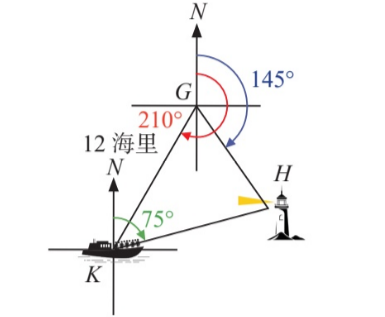
\includegraphics[width=0.5\textwidth]{S2_SUB/image.png}        
    \end{center}

    \begin{questionparts}
        \item 求海警船在点 $K$ 与港口 $H$ 的距离（精确至 $0.1$ 海里）； \qscore{6}

        \item 求由港口 $H$ 观测海警船在点 $K$ 的方位角（准确至 $1^{\circ}$）。 \qscore{3}

        \item 如图，摄影师布拉塞在点 $A$ 处，距巴黎铁塔底部 $D$ 的水平距离为 $200\ \mathrm{m}$，测得塔顶 $C$ 的仰角为 $58.3^{\circ}$。他想在仰角为 $45^{\circ}$ 处拍摄塔顶的结构细节，问他应向前走还是向后退，移动多少米？（忽略摄影师身高，答案准确至整数） \qscore{5}
        \begin{center}
            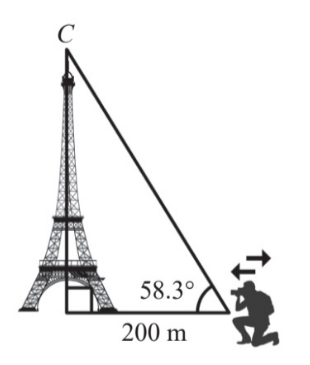
\includegraphics[width=0.5\textwidth]{S2_SUB/image_2.png}
        \end{center}
    \end{questionparts}
\end{question}

\begin{solution}
    \begin{enumerate}[label=(\alph*)]
        \item 求 $KH$ 的长。 \\
        由方位角求出 $\triangle GKH$ 的内角 $\angle KGH,\angle GKH$，再由内角和及正弦定律求 $KH$。 \\
        \begin{align*}
            \angle KGH &= 210^{\circ}-145^{\circ} = 65^{\circ}
        \end{align*}
        \begin{align*}
            \angle GKH &= 75^{\circ}-(210^{\circ}-180^{\circ}) = 45^{\circ}
        \end{align*}
        \begin{align*}
            \angle GHK &= 180^{\circ}-65^{\circ}-45^{\circ} = 70^{\circ}
        \end{align*}
        \begin{align*}
            \frac{KH}{\sin\angle KGH} &= \frac{GK}{\sin\angle GHK} \\
            KH &= \frac{12\sin65^{\circ}}{\sin70^{\circ}}
        \end{align*}
        \begin{align*}
            KH &\approx 11.6\ \text{海里}
        \end{align*}

        \item 求由 $H$ 观测 $K$ 的方位角。 \\
        过 $H$ 作正南北线，由南北线平行，内错角相等。 \\
        \begin{align*}
            \text{$HK$ 与正南方向的夹角} &= 75^{\circ}
        \end{align*}
        \begin{align*}
            \text{方位角} &= 180^{\circ}+75^{\circ} = 255^{\circ}
        \end{align*}

        \item 求摄影师为使塔顶仰角变为 $45^{\circ}$，应移动的方向与距离。 \\
        先在 Rt$\triangle ACD$ 中求塔高 $CD$；仰角为 $45^{\circ}$ 时，摄影师到塔底的水平距离等于塔高，再与 $200\ \mathrm{m}$ 比较。 \\
        设塔高 $CD=h$，则
        \begin{align*}
            \tan58.3^{\circ} &= \frac{h}{200}
        \end{align*}
        \begin{align*}
            h &= 200\tan58.3^{\circ} \approx 323.8\ \mathrm{m}
        \end{align*}
        设仰角为 $45^{\circ}$ 时，摄影师到塔底的水平距离为 $d$，则
        \begin{align*}
            \tan45^{\circ} &= \frac{h}{d} \\
            d &= h \approx 323.8\ \mathrm{m}
        \end{align*}
        因 $d>200\ \mathrm{m}$，故应向后退，
        \begin{align*}
            d-200 &\approx 323.8-200 \approx 124\ \mathrm{m}
        \end{align*}
    \end{enumerate}
\end{solution}
%endregion

\vfill % 与上方内容保持距离

\noindent
\newlength{\sigwidth}
\settowidth{\sigwidth}{（\hspace{4em}师）}

\begin{tabular*}{\textwidth}{@{\extracolsep{\fill}} l l l}
    出题： & 审题： & 审核： \\[4em]
    \rule{\sigwidth}{0.5pt} &
    \rule{\sigwidth}{0.5pt} &
    \rule{\sigwidth}{0.5pt} \\
    （\hspace{0em} \setterteacher ） &
    （\hspace{0em} \reviewteacher ） &
    （\hspace{0em} \auditteacher ） \\
\end{tabular*}

\newpage

\end{document}